\subsection{Melihat daftar laporan pengguna}
Halaman ini hanya dapat diakses oleh \textit{administrator} yang sebelumnya sudah login. Detail kasus penggunaan dapat dilihat tabel spesifikasi kasus penggunaan \ref{uc05.01}.\\
\indent Tidak ada \textit{view logic} ataupun logika \textit{UI} khusus dalam halaman ini. Kode sumber implementasi \textit{back-end} dapat dilihat pada kode sumber \ref{cdbe.05-01}.

\begin{lstlisting}[label=cdbe.05-01,style=php,caption=Kode Sumber Antarmuka Registrasi]

/** 
 * File : app/Http/Controllers/UserController
 * Menampilkan halaman daftar pengguna
 * langsung diFetch dari base Model User
 * Method : GET
 */
public function user()
{
    $data['data'] = User::paginate(20);
    return view('pages.user.index', $data);
}
\end{lstlisting}
      
  \begin{figure}[H]
    \centering
    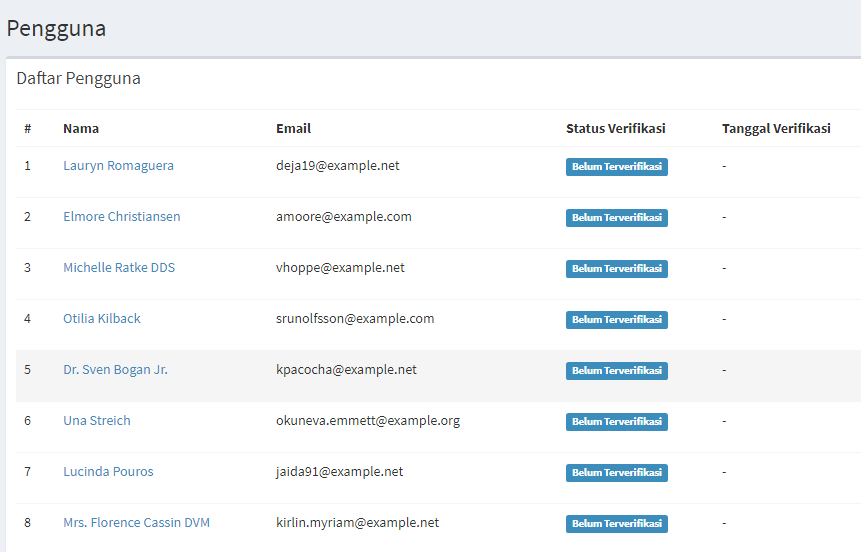
\includegraphics[width=\textwidth]{images/bab4/ui/05-01.png}
    \caption{Halaman Antarmuka Kasus Penggunaan Melihat Daftar Pengguna}
    \label{ui.05-01}
  \end{figure}
      
